\documentclass{article}
\usepackage{amsmath, amssymb, tikz}

\renewcommand{\L}{\mathcal{L}}

\begin{document}
\begin{flushleft}
Given $n \in \mathbb{N}_{\geq 3}$, consider the following quiver $Q_n$:
\begin{center}
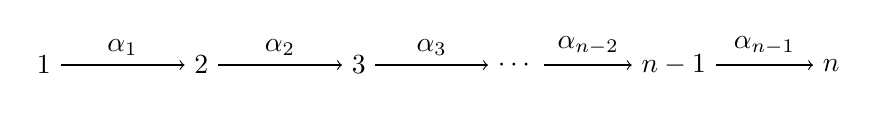
\begin{tikzpicture}
\node (A) at (0,0) {1};
\node (B) at (2,0) {2};
\node (C) at (4,0) {3};
\node (D) at (6,0) {$\cdots$};
\node (E) at (8,0) {$n-1$};
\node (F) at (10,0) {$n$};
\draw[->] (A) -- (B) node[midway, anchor=south] {$\alpha_1$};
\draw[->] (B) -- (C) node[midway, anchor=south] {$\alpha_2$};
\draw[->] (C) -- (D) node[midway, anchor=south] {$\alpha_3$};
\draw[->] (D) -- (E) node[midway, anchor=south] {$\alpha_{n-2}$};
\draw[->] (E) -- (F) node[midway, anchor=south] {$\alpha_{n-1}$};
\end{tikzpicture}
\end{center}
We let $\mathcal{L}_2$ denote the set of all non-zero length $2$ paths in $Q_n$. Hence,
\[
\mathcal{L}_2 := \left\{\alpha_i \alpha_{i+1} : 1 \leq i \leq n-2\right\}
\]
It clearly follows that $\left|\L_2\right| = n-2.$ \\[\baselineskip]

To introduce some new notation, we let 
\[\L_2^2 := \left\{(\alpha_i\alpha_{i+1}, \alpha_j\alpha_{j+1}) \; : \; i \neq j \text{ and } j > i\right\}.
\]
We require $j > i$ so that $(k, \ell) \in \L_2^2 \implies (\ell, k) \not\in \L_2^2$. \\
In other words, we are trying to enforce that $(k, \ell) = (\ell, k)$. \\[\baselineskip]

Next, we want to determine $\left|\L_2^2\right|$. Starting with $(\alpha_1, \ast)$, there are $n-3$
choices for $\ast$ since $|\L_2| = n-2$ and we cannot have $\ast$ be $\alpha_1$. For $\alpha_2$, 
there are $n-4$ choices for $\ast$ since $\ast$ cannot be $\alpha_1$ (since $j >i$) or $\alpha_2$.
Extending this, it then follows that 
\begin{align*}
   \left|\L_2^2\right| &= (n-3) + (n-4) + \ldots + 0 \\
                       &= \sum_{i=0}^{n-3} (n-3-i) \\
                       &= \sum_{i=0}^{n-3} n - \sum_{i=0}^{n-3} 3 - \sum_{i=0}^{n-3} i \\
                       &= n(n-3) - 3(n-3) - \frac{1}{2}(n-4)(n-3) \\
                       &= n^2 - 3n - 3n + 9 - \frac{1}{2}\left(n^2 - 7n + 12\right) \\
                       &= \frac{1}{2}(n-2)(n-3).
\end{align*}
Generalising, 
\begin{align}
   \left|\L_2^k\right| &= \sum_{i=0}^{n-(k+1)} n - 2 - (k - 1) - i \\
   &= \sum_{i=0}^{n-(k+1)} n - (k+1) - i \\
   &= \sum_{i=0}^{n-(k+1)} n - \sum_{i=0}^{n-(k+1)} (k+1) - \sum_{i=0}^{n-(k+1)} i \\
   &= n^2 - n(k+1) - n(k+1) + (k+1)^2 - \frac{1}{2}\left[n-(k+1)\right]\left(n-k\right) \\
   &= n^2 - 2n(k+1) + (k+1)^2 - \frac{1}{2}(n^2 - nk - nk - n + k^2 + k) \\
   &= n^2 - 2n(k+1) + (k+1)^2 - \frac{1}{2}\left[n^2 - 2nk - n + k(k+1)\right] \\
   &= \frac{1}{2}n^2 + nk - 2n(k+1) + (k+1)^2 + \frac{n}{2} - \frac{1}{2}k(k+1) \\
   &= \frac{1}{2}n^2 + nk - 2nk - 2n + (k+1)^2 + \frac{n}{2} - \frac{1}{2}k(k+1) \\
   &= \frac{1}{2}n^2 - nk - \frac{3}{2}n + (k+1)^2  - \frac{1}{2}k(k+1) \\
   &= \frac{1}{2}n(n - 2k - 3) + (k+1)^2  - \frac{1}{2}k(k+1) \\
   &= \frac{1}{2}n(n - 2k - 3) + (k^2 + 2k + 1)  - \frac{1}{2}(k^2 + k) \\
   &= \frac{1}{2}n(n - 2k - 3) + \frac{1}{2}k^2 + \frac{3}{2}k + 1 \\
   &= \frac{1}{2}n(n - 2k - 3) + \frac{1}{2}(k^2 + 3k + 2) \\
   &= \frac{1}{2}n(n - 2k - 3) + \frac{1}{2}(k+2)(k+1) \\
   &= \frac{1}{2}\left[n(n - 2k - 3) + (k+2)(k+1)\right].
\end{align}
\end{flushleft}
If $k=2$, we get
   \begin{align*}
      \frac{1}{2}\left[n(n-7) + 12\right] = \frac{1}{2}(n^2 - 7n + 12) = \frac{1}{2}(n-4)(n-3).
   \end{align*}
   some error. general result is 
   \[
      \left|\L_2^k\right| &= \sum_{i=0}^{n-(k+1)} n - 2 - (k - 1) - i = \frac{1}{2}(n-k)(n-(k+1))
   \]
\end{document}
